%standard 10.1

%start_of_questions


%new_question
%%%%%%%%%%%%%%%%%%%%%
	% Problem 1
	% Difficulty: 1
%%%%%%%%%%%%%%%%%%%%%
	\item 
		In Harry Potter, the currency consists of knuts, sickle, and galleon. There are 29 knuts in 
		one sickle and 17 sickles in one galleon. Write a \textbf{function} that will return a 
		converted amount of knuts into the fewest amount of coins possible. Only return a string 
		with the non-zero values, meaning don't return something similar to ``0 sickles''. The 
		argument for the function will be $knuts$ (how many knuts to convert), if no argument is 
		provided then the \textbf{default} should be 900 knuts. \\ \\
		\textbf{Debug this Solution:}\\
		\mbox{ \hspace*{0.25in}	\lstinputlisting[language=Python]{./code/debugger_p1_HarryPotter.py}}

%Error 1: default should be 900
%Error 2: remaining_knuts should use remainder \% not //
%Error 3: first if for galleons should be >
\pagebreak



%new_question
%%%%%%%%%%%%%%%%%%%%%
	% Problem 2
	% Difficulty: 1
%%%%%%%%%%%%%%%%%%%%%
	\item 
		Primary U.S. interstate highways are numbered 1-99 (Inclusive).  Odd numbers (like 5 or 95) go north/
		south, and evens (like 10 or 82) go east/west.  Auxiliary highways are numbered 100-999, and 
		service the primary highway indicated by the rightmost two digits.  Thus, I-405 services 
		I-5, and I-290 services I-90.
		
		Note: 200 is not a valid auxiliary highway because 00 is not a valid primary highway 
		number.\\
		
		Write a \textbf{function} that returns whether the highway runs north/south or east/west or is an 
		invalid highway number. The argument for the function 
		will be $highway\_num$(highway number provided). \\ \\
		\textbf{Debug this Solution:}\\
		\mbox{ \hspace*{0.25in}	\lstinputlisting[language=Python]{./code/debugger_p2_HighwayDirections.py}}

% Error 1: "if 1 > highway_num < 99" should be "if 1 <= highway_num <= 99"
% Error 2: In primary highways, the return strings for even/odd are swapped.
% Error 3: In the auxiliary highway service check, 'elif' should be 'else' because it incorrectly checks the same condition twice.
\pagebreak



%new_question
%%%%%%%%%%%%%%%%%%%%%
	% Problem 3
	% Difficulty: 1
%%%%%%%%%%%%%%%%%%%%%
	\item 
		%https://edabit.com/challenge/xR248CxGSsSrNK5Za
		You are the newest rug fashion designer on the scene, but you're running out of ideas. 
		Write a \textbf{function} that will help you design rugs.  The function will return a 
		formatted string that will resemble a designed rug. The first parameter must be $width$ 
		(how wide the rug will be), the second must be $length$ (how long the rug will be), 
		and the third must be $pattern$ (the character pattern used in the rug design).

		\textbf{Examples:} \\
			design\_run(3,5,\$) $\rightarrow$	\begin{tabular}{l}
			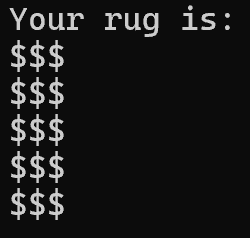
\includegraphics[height=1in]{./imgs/rug1_alt.PNG} \hspace{0.5in} \end{tabular}
			design\_run(16,5,\@) $\rightarrow$ \begin{tabular}{l}
			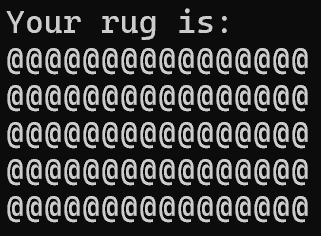
\includegraphics[height=1in]{./imgs/rug2_alt.PNG} \end{tabular}

		\textbf{Debug this Solution:}\\
		\mbox{ \hspace*{0.25in}	\lstinputlisting[language=Python]{./code/debugger_p3_Rugs.py}}

%Error 1: for i in range(length -1) should be for i in range(length)
%Error 2: pattern should be pattern ='@'
%Error 3: result += "\t" should be result += "\n"
\pagebreak



%new_question
%%%%%%%%%%%%%%%%%%%%%
	% Problem 4
	% Difficulty: 1
%%%%%%%%%%%%%%%%%%%%%
	\item 
		%https://edabit.com/challenge/b8wRDMWgMZTN2nmfx
		Write a \textbf{function} that returns the number of copies of the same number. 
		The arguments for the function will be $num\_1$ (first number), $num\_2$ (second number), 
		and $num\_3$ (third number).\\

		\textbf{Examples:}		
		\begin{itemize}
			\item  count\_duplicates(2, 3, 2) $\rightarrow$ \csq{You entered the same number 2 times}, 
			\item  count\_duplicates(4, 4, 4) $\rightarrow$ \csq{You entered the same number 3 times}, 
			\item  count\_duplicates(1, 2, 3) $\rightarrow$ \csq{Each number is unique} 
		\end{itemize}

		\textbf{Debug this Solution:}\\
		\mbox{ \hspace*{0.25in}	\lstinputlisting[language=Python]{./code/debugger_p4_NumberCopies.py}}

%Error 1: count should be 1
%Error 2: count = 1 should be count += 1
%Error 3: num_1 == num_3 is repeated twice
\pagebreak




%new_question
%%%%%%%%%%%%%%%%%%%%%
	% Problem 6
	% Difficulty: 1
%%%%%%%%%%%%%%%%%%%%%
	\item
		Write a function called \textit{flip\_flop} that takes a string as an argument 
		and returns a new word made up of the second half of the word first combined 
		with the first half of the word second.\\ 

		\textbf{Debug this Solution:}\\
		\mbox{ \hspace*{0.25in}	\lstinputlisting[language=Python]{./code/debugger_p6_FlipFlop.py}}

%Error 1: if length // 2 == 0: should be if length % 2 == 0:
%Error 2: first_half = word[middle:] should be first_half = word[:middle]
\pagebreak



%new_question
%%%%%%%%%%%%%%%%%%%%%
	% Problem 7
	% Difficulty: 1
%%%%%%%%%%%%%%%%%%%%%
	\item 
		The hamming distance is the number of characters that differ between two strings. 
		Write a function named hamming\_distance that takes two strings as arguments and 
		returns the hamming distance.\\
		
		\textbf{Debug this Solution:}\\
		\mbox{ \hspace*{0.25in}	\lstinputlisting[language=Python]{./code/debugger_p7_HammingDistance.py}}

%Error 1: distance = 1 should be distance = 0
%Error 2: for i in range(len(str1) -1): should be for i in range(len(str1) ):
%Error 3: if str1[i] == str2[i]: should be if str1[i] != str2[i]:
\pagebreak


%end_of_questions
%make sure to leave at least one blank line below

